\documentclass[a4paper,12pt]{report}
\usepackage[utf8]{inputenc}
\usepackage[T1]{fontenc}
\usepackage{graphicx}
\usepackage{geometry}
\usepackage{setspace}
\usepackage{titling}
\usepackage{fancyhdr}
\usepackage{ifthen}
\usepackage{lastpage}
\usepackage{xurl}  % Permet de casser les URL de manière améliorée
\usepackage[breaklinks]{hyperref}  % Permet de casser les liens URL
\def\UrlBreaks{\do\/\do-}
\usepackage[french]{babel}
\renewcommand\thesection{\Roman{section}} % Numérotation des sections en chiffres romains
\renewcommand\thesubsection{\arabic{subsection}} % Numérotation des sous-sections en chiffres arabes

% Pour gerer l'espace dans la table of contents
\usepackage{tocloft}
\renewcommand{\cftsecnumwidth}{2.3em} % Ajustez la largeur en fonction de vos besoins
\renewcommand{\cftsubsecnumwidth}{2.3em} % Ajustez la largeur en fonction de vos besoins
% ---

\hypersetup{
    colorlinks=true,
    linkcolor=black, % Couleur des liens internes (table des matières, etc.)
    urlcolor=blue, % Couleur des liens externes (URLs)
    citecolor=blue, % Couleur des liens de citation
    filecolor=blue % Couleur des liens vers des fichiers
}

\fancyhf{} % Efface les en-têtes et pieds de page par défaut
\pagestyle{fancy}
\renewcommand\headrulewidth{1pt}
\fancyhead[L]{Romain GALLAND | Quentin RADLO}
\fancyhead[R]{Université de Marie \& Louis Pasteur}
\renewcommand\footrulewidth{1pt}
\fancyfoot[L]{}
\fancyfoot[C]{Rapport de Projet - Simulateur de conduite:\\
\textbf{Page \thepage/\pageref{LastPage}}}
\fancyfoot[R]{}
\geometry{
  bindingoffset=1cm,  % Décalage pour la reliure
  left=2cm,
  right=2cm,
  top=2.5cm,
  bottom=2.5cm
}

\setlength{\headheight}{14.5pt}
\addtolength{\topmargin}{-2.5pt}

\begin{document}

\begin{titlepage}

 \begin{center}
    \vspace{2cm}
    
\includegraphics[width=0.3\textwidth]{university_logo.png}\par
  \end{center}



  \begin{center}
    \vspace{0.2cm}
    {\scshape \large{Rapport de projet} \par}
    Licence 3 Informatique - UFR Sciences et Techniques
    \vspace{0.4cm}
    \hrule
    \vspace{0.4cm}
    {\huge\bfseries Simulateur de conduite \par}
    \vspace{0.4cm}
    \hrule
    \vspace{1cm}
    {\large\bfseries Décembre 2024 - Mars 2025 \par}
    Romain GALLAND - Quentin RADLO
    %\vspace*{1.5cm}
 % Image d'illustration
    % \vspace*{1.5cm}
    \vspace{1cm} % Fonctionne mieux si encapsulé dans un bloc centre
    \begin{center}
        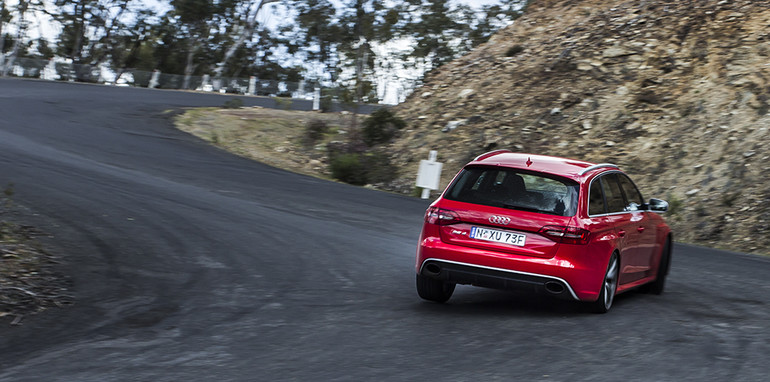
\includegraphics[width=0.8\textwidth]{illustration.jpg}
    \end{center}


    % Informations supplémentaires
    \vspace{1cm}
    {\bfseries Sous la supervision de:} Jean-Michel Hufflen \\


  \end{center}
\end{titlepage}


\newpage
\section*{Remerciements}
- Un remerciement particulier est adressé à M. Hufflen pour la guidance et la pédagogie qu'il nous a apporté lors de la réalisation de notre projet.

% Page dédiée à la table des matières
\newpage
\tableofcontents
\newpage


\newpage
\section*{Glossaire}

\textbf{APEC :} Agence pour l'Emploi des Cadres, une association française qui propose des offres d'emploi pour les cadres.

\textbf{Bluetooth :} Norme de communication sans fil à courte portée.

\textbf{C, C++ :} Langages de programmation populaire dans le milieu embarqué.

\textbf{ESP32 :} Microcontrôleur très utilisé dans le développement de projets embarqués.

\textbf{Framework :} Ensemble d'outils et de conventions facilitant le développement.

\textbf{Git :} Système de gestion de versions décentralisé.

\textbf{I2C :} Protocole de communication entre plusieurs dispositifs.

\textbf{LinkedIn :} Réseau social professionnel en ligne.

\textbf{OS :} Système d'exploitation (\textit{Operating System} en anglais).

\textbf{RTOS :} Système d'exploitation temps réel (\textit{Real-Time Operating System} en anglais).

\textbf{SPI :} Protocole de communication série synchrone utilisé principalement pour la communication entre microcontrôleurs et périphériques.

\textbf{SS2I :} Société de Services en Ingénierie Informatique.

\newpage
\section{Sujet du projet}

\subsection{Le sujet}
Le sujet originel nous laissait une assez grande liberté quant à l'orientation de notre projet. L'idée globale consistait en la réalisation graphique d'un mini-simulateur de conduite, avec des ordres de conduite (démarrage, arrêt, accélération et décélération) donnés par la frappe du clavier. L'utilisateur devait pouvoir observer son véhicule ainsi que le circuit avec une vue du dessus ou la vision du conducteur à travers le pare-brise. Il était aussi proposé de pouvoir "corser" le jeu en programmant des événements aléatoires.

Pour réaliser ce projet, plusieurs langages de programmation nous étaient proposés :
\begin{itemize}
    \item \textbf{DrRacket}, avec des compléments pour nous aider sur la partie graphique.
    \item \textbf{JRuby}, avec pour idée d'implémenter la logique du programme en Ruby et la partie graphique avec des bibliothèques de Java.
    \item \textbf{C\#} ou \textbf{C++} avec les bibliothèques graphiques adéquates.
\end{itemize}


\subsection{Notre interprétation du sujet / Objectif du sujet }
Après réflexion et discussion avec notre tuteur, nous avons décidé de partir vers une orientation didacticiel plutôt qu'une "orientation de 'jeu' ". L'idée était d'implémenter un modèle de dynamique de véhicule se rapprochant de la réalité. Avec un tel modèle, nous pourrions donc visualiser des comportements de perte d'adhérence sur la route, ainsi que les phénomènes de survirage et sous virage. Un tel simulateur permettrait donc à l'utilisateur d'expérimenter / se familiariser avec de tels comportements de véhicule. De ce qui est du langage de programmation, nous avons décidé de nous orienter vers le langage C++, car il nous était plus familier que les autres langages proposés, et nous avons utilisé SFML en tant que bibliothèque graphique.
Ensuite, nous avons donc commencé l'implémentation de notre simulateur, il s'est décomposé en deux grandes parties, l'implémentation de la physique et la création de l'interface graphique. Nous allons commencer par vous présenter la partie physique de notre projet.

\newpage

\section{L'implémentation de la physique / Modélisation d'un système de dynamique de véhicule}

\subsection{Introduction}
Pour représenter la relation entre un véhicule et la route d'une manière se rapprochant de la réalité, nous avons donc dû implémenter des phénomènes physiques venant des sciences de l'ingénieur. De plus, comme l'étude et la représentation d'un système  de dynamique de véhicule est une tâche plutôt difficile, nous avons décidé de procéder de manière itérative. Tout d'abord, le but était d'avoir une implémentation très basique d'un système de dynamique,  puis une fois celui-ci fonctionnel, d'itérer ce système pour intégrer des phénomènes plus délicats à implémenter, puis d'encore itérer sur ce système, etc.
Ceci nous a mené à un plan en 5 étapes.
Premièrement, implémenter les lois de Newton pour la dynamique du véhicule, puis implémenter un modèle bicycle simplifié, pour ensuite pouvoir représenter les forces sur les pneus et modéliser les glissements, et finalement pouvoir simuler les limites du pneumatique.
Nous allons maintenant vous détailler les principes physiques et l'implémentation, que nous avons fournis pour chacune de ces étapes :

\subsection{Implémentation des lois de Newton pour la dynamique du véhicule}

\begin{thebibliography}{99}
  \bibitem{interview}
    Abdallah Ben Othman,
    Interview réalisée le 10 Décembre 2023.

  \bibitem{CreditPhoto}
    \emph{Crédit photo :}
    \url{https://www.it-connect.fr/plus-dun-million-de-raspberry-pi-commercialises/},
    Florian Burnel, sous licence BY-NC-ND 4.0

  \bibitem{APEC}
    \emph{APEC - Offres d'emploi},
    \url{https://www.apec.fr/candidat.html},
    Consulté le 5 Décembre 2023.

  \bibitem{apec}
    \emph{APEC - Fiche Métier},
    \url{https://www.apec.fr/tous-nos-metiers/informatique/ingenieur-en-etudes-et-developpement-informatiques.html},
    Consulté le 19 novembre 2023.

  \bibitem{qt}
    \emph{QT},
    \url{https://www.qt.io/embedded-development-talk/embedded-engineers-roles-responsibilities-and-job-descriptions},
    Consulté le 2 Décembre 2023.

  \bibitem{kicklox}
    \emph{Kicklox},
    \url{https://www.kicklox.com/blog-talent/developpeur-logiciel-embarque},
    Consulté le 2 Décembre 2023.

  \bibitem{yuhiro}
    \emph{Yuhiro},
    \url{https://www.software-developer-india.com/fr/developpeur-de-logiciels-embarques-que-fait-il/},
    Consulté le 2 Décembre 2023.

  \bibitem{ti}
    \emph{Texas Instruments\\},
    \url{https://news.ti.com/blog/2023/04/07/3-trends-impacting-future-embedded-processing-technology},
    Consulté le 12 décembre 2023.

  \bibitem{readwrite}
    \emph{ReadWrite},
    \url{https://readwrite.com/embedded-systems-and-the-future/},
    Consulté le 12 décembre 2023.

\end{thebibliography}
\end{document}